% An example https://godbolt.org/z/h4rv6Y6G9
\begin{frame}[fragile]
\raggedright
\frametitle{A motivating example}

\begin{itemize}
    \item \textbf{Aliasing}: different symbolic names refer to the same object
    \item \textbf{Pointee}: the object pointed to by a pointer
\end{itemize}

\leavevmode\\

\begin{minted}[escapeinside=||,mathescape=true,linenos,texcomments]{c}
int foo1(int* p, int* q) {   
    *p = 10;
    *q = 11;
    return *p; // if $p$ and $q$ do not alias, $*p$ must evaluate to $10$
               // if $p$ and $q$ alias, $*p$ must evaluate to $11$
}
\end{minted}

\end{frame}

\begin{frame}[fragile]
\raggedright
\frametitle{A motivating example}

\begin{itemize}
    \item \textbf{Restrict}: programmer-provided information to inform the compiler specific pointers do not alias under certain conditions
\end{itemize}

\leavevmode \\

\begin{minted}[escapeinside=||,mathescape=true,linenos,texcomments]{c}
// \colorbox{blue!20}{Programmer}: hi compiler! I promise you $p$ and $q$ will not alias
int foo2(int* |\colorbox{blue!20}{restrict}| p, int* |\colorbox{blue!20}{restrict}| q) {
    *p = 10;
    *q = 11;
    return *p; // if $p$ and $q$ do not alias, $*p$ must evaluate to $10$
               // if $p$ and $q$ alias, $*p$ must evaluate to $11$
}
\end{minted}

\begin{figure}
\centering
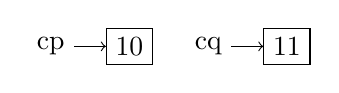
\begin{tikzpicture}
    \node (p) {\mintinline{c}{p}};
    \node[right of = p, draw, rectangle] (pointee-p) {$10$};

    \node[right of = pointee-p] (q) {\mintinline{c}{q}};
    \node[right of = q, draw, rectangle] (pointee-q) {$11$};

    \draw[->] (p) -- (pointee-p);
    \draw[->] (q) -- (pointee-q);
\end{tikzpicture}
\end{figure}

\end{frame}


\begin{frame}[fragile]
\raggedright
\frametitle{A motivating example}
\begin{minted}[escapeinside=||,mathescape=true,linenos,texcomments]{c}
// \colorbox{blue!20}{Programmer}: hi compiler! I promise you $p$ and $q$ will not alias
// \colorbox{orange!20}{Compiler}: nice! Thanks to this information, I optimized your code
int foo2_optimized(int* |\colorbox{blue!20}{restrict}| p, int* |\colorbox{blue!20}{restrict}| q) {   
    *p = 10;
    *q = 11;
    return |\colorbox{orange!20}{\soutthick{*p} 10}|;
}

\end{minted}

\begin{figure}
\centering
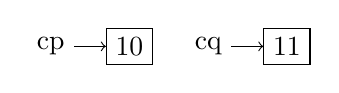
\begin{tikzpicture}
    \node (p) {\mintinline{c}{p}};
    \node[right of = p, draw, rectangle] (pointee-p) {$10$};

    \node[right of = pointee-p] (q) {\mintinline{c}{q}};
    \node[right of = q, draw, rectangle] (pointee-q) {$11$};

    \draw[->] (p) -- (pointee-p);
    \draw[->] (q) -- (pointee-q);
\end{tikzpicture}
\end{figure}

\end{frame}

\begin{frame}[fragile]
\raggedright
\frametitle{The promise can be broken}
\begin{minipage}{0.4\textwidth}
\begin{minted}[escapeinside=||,mathescape=true,texcomments]{c}
int foo1(int* p, int* q) {   
    *p = 10;
    *q = 11;
    return *p;
}
\end{minted}
\end{minipage}%
\begin{minipage}{0.6\textwidth}
\begin{minted}[escapeinside=||,mathescape=true,texcomments]{c}
int foo2(int* |\colorbox{blue!20}{restrict}| p, int* |\colorbox{blue!20}{restrict}| q) {   
    *p = 10;
    *q = 11;
    return |\colorbox{orange!20}{\soutthick{*p} 10}|;
}
\end{minted}
\end{minipage}

\pause

\begin{minted}[escapeinside=||,mathescape=true,linenos,texcomments]{c}
int main() {
    int x;
    printf("%d, %d\n", foo1(&x, &x), foo2(&x, &x));
}
\end{minted}

\begin{figure}
\centering
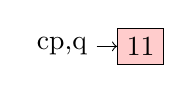
\begin{tikzpicture}
    \node (p) {\mintinline{c}{p,q}};
    \node[right of = p, draw, rectangle, fill=red!20] (pointee) {$11$};

    \draw[->] (p) -- (pointee);
\end{tikzpicture}
\end{figure}

\begin{itemize}
    \item Prints $11, 10$, \ie the optimized code has a different result than the original code
    \item Is the optimization incorrect?
\end{itemize}

\end{frame}
